\documentclass[journal]{vgtc}                % final (journal style)
%\documentclass[review,journal]{vgtc}         % review (journal style)
%\documentclass[widereview]{vgtc}             % wide-spaced review
%\documentclass[preprint,journal]{vgtc}       % preprint (journal style)

%% Uncomment one of the lines above depending on where your paper is
%% in the conference process. ``review'' and ``widereview'' are for review
%% submission, ``preprint'' is for pre-publication, and the final version
%% doesn't use a specific qualifier.

%% These few lines make a distinction between latex and pdflatex calls and they
%% bring in essential packages for graphics and font handling.
%% Note that due to the \DeclareGraphicsExtensions{} call it is no longer necessary
%% to provide the the path and extension of a graphics file:
%% 
\includegraphics{diamondrule} is completely sufficient.
%%
\ifpdf%                                % if we use pdflatex
  \pdfoutput=1\relax                   % create PDFs from pdfLaTeX
  \pdfcompresslevel=9                  % PDF Compression
  \pdfoptionpdfminorversion=7          % create PDF 1.7
  \ExecuteOptions{pdftex}
  \usepackage{graphicx}                % allow us to embed graphics files
  \DeclareGraphicsExtensions{.pdf,.png,.jpg,.jpeg} % for pdflatex we expect .pdf, .png, or .jpg files
\else%                                 % else we use pure latex
  \ExecuteOptions{dvips}
  \usepackage{graphicx}                % allow us to embed graphics files
  \DeclareGraphicsExtensions{.eps}     % for pure latex we expect eps files
\fi%

%% it is recomended to use ``\autoref{sec:bla}'' instead of ``Fig.~\ref{sec:bla}''
\graphicspath{{figures/}{pictures/}{images/}{./}} % where to search for the images

\usepackage{microtype}                 % use micro-typography (slightly more compact, better to read)
\PassOptionsToPackage{warn}{textcomp}  % to address font issues with \textrightarrow
\usepackage{textcomp}                  % use better special symbols
\usepackage{mathptmx}                  % use matching math font
\usepackage{times}                     % we use Times as the main font
\renewcommand*\ttdefault{txtt}         % a nicer typewriter font
\usepackage{cite}

%% If you are submitting a paper to a conference for review with a double
%% blind reviewing process, please replace the value ``0'' below with your
%% OnlineID. Otherwise, you may safely leave it at ``0''.
\onlineid{0}

%% declare the category of your paper, only shown in review mode
\vgtccategory{Research}

%% Paper title - 1 pt for descriptive title
\title{The title for your project.}

%% This is how authors are specified in the journal style

%% indicate IEEE Member or Student Member in form indicated below
%% 1 pt for name
\author{Your Name Here}
\authorfooter{
%% insert punctuation at end of each item
\item
 Your Name is a graduate student at the University of Arizona. E-mail:[your
 NetID]@email.arizona.edu.
}

%other entries to be set up for journal
%\shortauthortitle{Firstauthor \MakeLowercase{\textit{et al.}}: Paper Title}

%% Abstract section - 5 pts
\abstract{
Abstract goes here. Summarize the project, why it is important, what you
plan to do, and what the community may learn from this in 150-250 words.

} % end of abstract

%% Keywords that describe your work. Will show as 'Index Terms' in journal
%% please capitalize first letter and insert punctuation after last keyword
%\keywords{Radiosity, global illumination, constant time}

%% ACM Computing Classification System (CCS). 
%% See <http://www.acm.org/class/1998/> for details.
%% The ``\CCScat'' command takes four arguments.

%\CCScatlist{ % not used in journal version
% \CCScat{K.6.1}{Management of Computing and Information Systems}%
%{Project and People Management}{Life Cycle};
% \CCScat{K.7.m}{The Computing Profession}{Miscellaneous}{Ethics}
%}

%% Uncomment below to include a teaser figure.
%   \teaser{
%   \centering
%   \includegraphics[width=16cm]{CypressView}
%   \caption{In the Clouds: Vancouver from Cypress Mountain.}
%  }

%% Uncomment below to disable the manuscript note
%\renewcommand{\manuscriptnotetxt}{}

%% Copyright space is enabled by default as required by guidelines.
%% It is disabled by the 'review' option or via the following command:
% \nocopyrightspace

\vgtcinsertpkg

%%%%%%%%%%%%%%%%%%%%%%%%%%%%%%%%%%%%%%%%%%%%%%%%%%%%%%%%%%%%%%%%
%%%%%%%%%%%%%%%%%%%%%% START OF THE PAPER %%%%%%%%%%%%%%%%%%%%%%
%%%%%%%%%%%%%%%%%%%%%%%%%%%%%%%%%%%%%%%%%%%%%%%%%%%%%%%%%%%%%%%%%

\begin{document}

%% The ``\maketitle'' command must be the first command after the
%% ``\begin{document}'' command. It prepares and prints the title block.

%% the only exception to this rule is the \firstsection command
\firstsection{Introduction} % or "Motivation"

\maketitle

% Introduction and/or Motivation - 20%

Strongly motivate your project in this section.

Summarize the problem you are trying to solve.

Explain why the problem is important -- who benefits from the problem being
solved and in what way? If the problem were to be solved, what would that
enable people to do?

Summarize what you plan to do to solve the problem.

% You may want to end this section by summarizing it again as a list, for example:
The aims of this research are:
\begin{itemize}
  \item a taxonomy of tasks performed in the visual analysis of octopi 
  \item developing a new technique for visualizing octopi
  \item a validated visual design supporting the visual analysis of octopi
\end{itemize}

 

%Background and Related Work: 20%

\section{Background}
\label{sec:background}

Expand on what the reader needs to know and understand if it necessary to
adequately describe the problem. This may include definitions of terms and
explanations of the present workflow people use to solve the task.

This section should answer the question "What does someone unfamiliar with the
area need to know to understand this project?" Often times this section focuses
on the \textit{domain}. For example, a new visualization for biology data will
explain the type of biology data used, the terminology that will be used to
describe it, the people who use it, and what they hope to learn from it. If
there is no specific domain, the background section may describe general terms
about the data abstraction (e.g. "We define a graph $G = (V, E)$ as..."),
common practices, or other information for visualization researchers who are
not as familiar with this problem in comparison to all the others. 

\subsection{Related Work}
\label{sec:related}

Discuss the work related to your project---include both visualization and
domain-specific references to the problem you're trying to solve. Prominent
related works should be included for this milestone. If you are proposing a
literature review or task taxonomy, this section must include a discussion of
what similar ones exist already and should tie into the motivation. Is the
existing one old enough to be missing many relevant advances?

For example, if my project involves analyzing performance data of distributed
systems, I might want to cite Perfopticon~\cite{Moritz:2015:EuroVis}. If my
project involves designing a new library to support creating new
visualizations, I might want to cite d3js~\cite{d3js}. Note here I am using
keys such as "Moritz:2015:EuroVis" for citations. These refer to the full
definitions in proposal.bib.

ACM Digital Library makes it easy to get bib files for proposal.bib and there
are guides online for citing things like books~\cite{ware:2004:IVP},
theses~\cite{levoy:1989:DSV}, journal articles~\cite{Lorensen:1987:MCA}, and
conference proceedings~\cite{Nielson:1991:TAD}. There's even a format for
miscellaneous references (misc) such as websites and libraries not associated
with a article.



%Research Plan - 20%
\section{Research Plan} 
\label{sec:research}

Re-state the problem you are trying to solve and then explain how you plan to solve it. Is it designing a new visualization? Is it designing a new library?  Is it running a controlled experiment? Is it something else?

Note this is a {\em plan}. The plan may change as you make discoveries during your project. However, you must describe what your plan is assuming everything goes as expected. If there are some parts of the plan where you could run into difficulties, state what those difficulties are and what alternative measures you could take should those difficulties arise.

You may refer to other sections so as not to repeat yourself -- for example, referencing Section~\ref{sec:background}.

You may want to use figures to illustrate your point, such as Figure~\ref{fig:sample}.

\begin{figure}[h]
 \centering % avoid the use of \begin{center}...\end{center} and use \centering instead (more compact)
 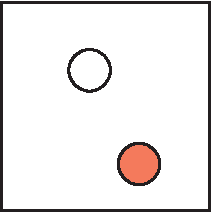
\includegraphics[width=1.5in]{figs/sample}
 \caption{Figure illustrating some proposed designs.}
 \label{fig:sample}
\end{figure}

\subsection{Data}
\label{sec:data}

Describe the data here. Describe whether you already have access to the data and if not, what is required to obtain the data. If you don't already have the data, explain how long it will take to retrieve it. 

\subsection{Evaluation}
\label{sec:eval}

Describe your plan for evaluating your work during this project.

Then, describe how you would evaluate the work beyond the timeframe of the project. Without time constraints, what would you do? Do you have the resources (people, time, equipment, data, money) to implement this plan in the future? Does your plan for evaluating your work during the project serve as a first step to this evaluation?

\subsection{Technology}
\label{sec:tech}

Describe what technologies you intend to use (e.g., programming languages, platforms, existing libraries) and why they make sense for your project. Do they serve your users better than other technologies? Are you able to take advantage of existing work/libraries for your domain with this technology rather than HTML/CSS/JS and d3.js?  

\subsection{Timeline}
\label{sec:timeline}

Adapt the milestones for the class project to the specifics of your project, describe them in this section, and summarize in Table~\ref{tab:milestones}.  You may set intermediate milestones, but you should make it clear what you will have accomplished by the progress update milestone (due Oct. 29, 2020).  Use paragraphs to make it clear what the milestone means, for example:

\paragraph{Milestone 1} Description

\paragraph{Milestone 1} Description

These milestones can include many subgoals.  If you are developing a new technique or visualization, you should have a preliminary idea of the design.  You may want to consider developing a prototype or preliminary design by the progress update step.  Any data needed to support initial findings or background work should be cited and discussed.  If you are doing a literature review or taxonomy, you should have a preliminary list of papers you will review as well as an explanation of the methodology used to generate such a list.  If your evaluation requires scaffolding code to run things, or human subjects to test things, you can describe when you will set these up.

By the progress update stage, there should be initial results of the first chunk of work that needs to be done.  In most projects with implementation this will involve a working data reader and at least one visualization, library feature, or study question type working. As you will need a report at this stage, be sure to set up milestones that will provide you with sufficient material to develop your report and update your plan, if necessary.   The demonstration should run with minimal effort and the code should be included in the repository.

Later milestones (after the progress update stage) can include a variety of stages included a complete prototype of the project artifacts,  such as a visualization tool, a visualization library, a working study with experimental objects and stimuli complete, or completed literature annotations with an categorization schema. The plan for evaluation especially should be updated indicating the plan for milestone five and any preliminary work in the design of that evaluation.


Additionally, a full report of the project as a whole should be included as a milestone.



\begin{table}[h]
%% Table captions on top in journal version
 \caption{Project Milestones}\vspace{1ex} % the \vspace adds some space after the top caption
 \label{tab:milestones}
 \scriptsize
 \centering % avoid the use of \begin{center}...\end{center} and use \centering instead (more compact)
   \begin{tabular}{r|r}
     Milestone & Description (\%)\\
   \hline
     Date & Summary Description \\
     Date & Summary Description \\
     October 29 & Progress Update \\
     Date & Summary Description \\
     December 8 & Final Report Completed \\
   \end{tabular}
\end{table}



% Impact - 20%
\section{Impacts}
\label{sec:impact}

Summarize the impact completing this work will have. This ties into why the
work is important and should relate to the motivation in the introduction.
What would be possible if this work was completed? Why is this work of interest
to the scientific community and the visualization community?


%\bibliographystyle{abbrv}
\bibliographystyle{abbrv-doi-hyperref}
%%use following if all content of bibtex file should be shown
%\nocite{*}
\bibliography{proposal}
\end{document}

